% Provenance (never printed): cycle 3 geography and "La planete Terre"
% (the great physical features of the world: relief, rivers, deserts, ice;
% reading a physical map); see sources/book1/PROVENANCE.md.
% Book 1, grade 4, chapter 3.
\chapter{O mapa físico do mundo}\label{ch:g4:world-physical-map}

Sami e Noor desdobram um grande \omterm{def:g2:drawing-to-map:map}{mapa} do mundo no chão da sala de aula e se
ajoelham em volta dele. Não é como os \omterm{def:g2:drawing-to-map:map}{mapas} que eles conhecem. Não há
países, nem fronteiras, nem cidades. Em vez disso, a terra está pintada de
cores: verde ao longo das costas e nas grandes terras planas, depois amarelo
claro, depois marrom e, em alguns lugares, quase branco. O \omterm{def:g2:water-on-earth:ocean}{mar} também tem
vários azuis: claro perto das costas, cada vez mais escuro longe, no meio
dos \omterm{def:g2:water-on-earth:ocean}{oceanos}.

``Por que aquela parte da Ásia é branca?'', pergunta Noor. ``É \omterm{def:g4:clouds-rain-snow:precipitation}{neve}?'' Não
exatamente. Neste \omterm{def:g2:drawing-to-map:map}{mapa}, cada cor diz a altura da terra, ou a profundidade do \omterm{def:g2:water-on-earth:ocean}{mar}.

\begin{recall}
Um \omterm{def:g2:drawing-to-map:map}{mapa} mostra um lugar visto de cima, feito menor; a sua \omterm{def:g2:drawing-to-map:legend}{legenda} explica
as cores e os símbolos (\cref{ch:g2:drawing-to-map}). As terras estão
reunidas em sete \omterm{def:g3:continents-and-oceans:continent}{continentes}, entre cinco \omterm{def:g2:water-on-earth:ocean}{oceanos}, e um \omterm{def:g3:continents-and-oceans:world-map}{mapa-múndi} é um
\omterm{def:g3:continents-and-oceans:globe}{globo} achatado (\cref{ch:g3:continents-and-oceans}). \omterm{def:g1:landscapes-around-us:landform}{Montanhas}, \omterm{def:g1:landscapes-around-us:landform}{colinas},
\omterm{def:g1:landscapes-around-us:landform}{vales} e \omterm{def:g1:landscapes-around-us:landform}{planícies} são as \omterm{def:g1:landscapes-around-us:landform}{formas de relevo}; os \omterm{def:g1:landscapes-around-us:water}{rios} correm das terras altas
até o \omterm{def:g2:water-on-earth:ocean}{mar} (\cref{ch:g1:landscapes-around-us}).
\end{recall}

\section{Ler um mapa físico}

Para dizer a que altura fica um lugar, precisamos de um nível de partida,
o mesmo em toda a Terra. Usamos o \omterm{def:g4:world-physical-map:altitude}{nível do mar}.

\begin{definition}[Altitude e nível do mar]\label{def:g4:world-physical-map:altitude}
O \emph{nível do mar}\index{nivel do mar@nível do mar} é o nível médio da superfície do
\omterm{def:g2:water-on-earth:ocean}{mar}, entre a maré alta e a maré baixa. A \emph{altitude}\index{altitude} de
um lugar é a sua altura acima do nível do \omterm{def:g2:water-on-earth:ocean}{mar}, em metros. Embaixo do \omterm{def:g2:water-on-earth:ocean}{mar},
falamos de \emph{profundidade}: a distância a que o fundo do \omterm{def:g2:water-on-earth:ocean}{mar} fica
abaixo do nível do \omterm{def:g2:water-on-earth:ocean}{mar}.
\end{definition}

Uma cidade à \omterm{def:g2:water-on-earth:ocean}{beira-mar} tem uma \omterm{def:g4:world-physical-map:altitude}{altitude} de poucos metros. Uma vila nas
\omterm{def:g1:landscapes-around-us:landform}{montanhas} pode ficar a 1\,500 metros: um quilômetro e meio acima do \omterm{def:g4:world-physical-map:altitude}{nível
do mar}, mesmo estando a centenas de quilômetros de qualquer costa.

\begin{definition}[Relevo]\label{def:g4:world-physical-map:relief}
O \emph{relevo}\index{relevo} de uma região é a forma do seu terreno: onde
ele é alto e onde é baixo, as suas \omterm{def:g1:landscapes-around-us:landform}{montanhas}, planaltos, \omterm{def:g1:landscapes-around-us:landform}{vales} e
\omterm{def:g1:landscapes-around-us:landform}{planícies}.
\end{definition}

\begin{definition}[Mapa físico]\label{def:g4:world-physical-map:physical-map}
Um \emph{mapa físico}\index{mapa fisico@mapa físico} mostra o \omterm{def:g4:world-physical-map:relief}{relevo} da terra e a
profundidade do \omterm{def:g2:water-on-earth:ocean}{mar} com cores, uma cor para cada faixa de \omterm{def:g4:world-physical-map:altitude}{altitude} ou de
profundidade, além dos grandes \omterm{def:g1:landscapes-around-us:water}{rios}, \omterm{def:g1:landscapes-around-us:water}{lagos}, desertos e gelos.
\end{definition}

\begin{omfigure}
\begin{tikzpicture}
\begin{axis}[ommap, width=\linewidth, xtick=\empty, ytick=\empty, grid=none,
    axis background/.style={}, clip=true]
  \addplot graphics[xmin=-180, xmax=180, ymin=-90, ymax=90]
    {figdata/out/grade-4-physical_map.png};
  \addplot[black!45, line width=0.15pt] table {figdata/out/shared-geo-land.dat};
  \addplot[fill=omHypsSeaB, draw=blue!60!black, line width=0.2pt]
    table {figdata/out/grade-4-physical_map-lakes.dat};
  \addplot[blue!70!black, line width=0.5pt] table {figdata/out/grade-4-physical_map-rivers.dat};
  \begin{scope}[every node/.style={font=\scriptsize\bfseries, align=center,
      fill=white, fill opacity=0.7, text opacity=1, inner sep=1pt, rounded corners=1pt}]
    \node at (axis cs:-112,47) {Montanhas\\Rochosas};
    \node at (axis cs:-62,-22) {Andes};
    \node at (axis cs:10,49) {Alpes};
    \node at (axis cs:84,24) {Himalaia};
    \node at (axis cs:4,23) {Saara};
    \node at (axis cs:-40,74) {Groenlândia\\(gelo)};
    \node at (axis cs:60,-80) {Antártida (gelo)};
  \end{scope}
  \begin{scope}[every node/.style={font=\scriptsize\itshape, text=blue!50!black,
      fill=white, fill opacity=0.6, text opacity=1, inner sep=1pt}]
    \node at (axis cs:38,17) {Nilo};
    \node at (axis cs:-56,-7) {Amazonas};
    \node at (axis cs:-80,33) {Mississípi};
    \node at (axis cs:118,26) {Yang-Tsé};
  \end{scope}
\end{axis}
\end{tikzpicture}

\smallskip
\begin{tikzpicture}[font=\scriptsize, x=1.18cm]
  \foreach \i/\c/\t in {0/5A9CCF/{abaixo\\de 4000}, 1/84BCE0/{2000\\a 4000},
      2/B3D8EE/{200\\a 2000}, 3/DCEEF8/{0\\a 200}} {
    \definecolor{tmp}{HTML}{\c}
    \fill[tmp, draw=black!40] (\i,0) rectangle (\i+0.92,0.35);
    \node[align=center, anchor=north] at (\i+0.45,-0.05) {\t};
  }
  \foreach \i/\c/\t in {5/9CC98A/{0\\a 200}, 6/C9DE99/{200\\a 500},
      7/F1E7A8/{500\\a 1000}, 8/E5C58A/{1000\\a 2000}, 9/C79E76/{2000\\a 4000},
      10/ECE8E3/{acima\\de 4000}} {
    \definecolor{tmp}{HTML}{\c}
    \fill[tmp, draw=black!40] (\i,0) rectangle (\i+0.92,0.35);
    \node[align=center, anchor=north] at (\i+0.45,-0.05) {\t};
  }
  \node[anchor=south] at (2,0.4) {profundidade do mar (m)};
  \node[anchor=south] at (8,0.4) {altitude da terra (m)};
\end{tikzpicture}

{\small O \omterm{def:g4:world-physical-map:physical-map}{mapa físico} do mundo, com a sua \omterm{def:g2:drawing-to-map:legend}{legenda}. Cada cor é uma faixa de
\omterm{def:g4:world-physical-map:altitude}{altitude} (na terra) ou de profundidade (embaixo do \omterm{def:g2:water-on-earth:ocean}{mar}). Os \omterm{def:g1:landscapes-around-us:water}{rios} estão em
azul-escuro. O \omterm{def:g4:world-physical-map:relief}{relevo} foi desenhado a partir de um valor a cada grau de
latitude e de longitude (cerca de a cada 100 quilômetros); por isso ele
está suavizado: picos isolados e fossas estreitas não aparecem. Dados:
relevo NOAA ETOPO1; \omterm{def:g1:landscapes-around-us:water}{rios}, \omterm{def:g1:landscapes-around-us:water}{lagos} e contornos das costas: Natural Earth.}
\label{fig:g4:world-physical-map:map}
% ledger: data:etopo1, data:b1-ne-rivers, data:ne-land
\end{omfigure}

\begin{method}[Ler uma cor num mapa físico]\label{met:g4:world-physical-map:reading}
Para achar a \omterm{def:g4:world-physical-map:altitude}{altitude} de um lugar num \omterm{def:g4:world-physical-map:physical-map}{mapa físico}:
\begin{enumerate}
  \item encontre o lugar e observe a sua cor;
  \item encontre a mesma cor na \omterm{def:g2:drawing-to-map:legend}{legenda};
  \item leia a faixa embaixo dela: a \omterm{def:g4:world-physical-map:altitude}{altitude} do lugar fica entre os dois
        números.
\end{enumerate}
No \omterm{def:g2:water-on-earth:ocean}{mar}, a profundidade se lê do mesmo jeito.
\end{method}

\begin{example}[Três lugares]\label{ex:g4:world-physical-map:three}
A foz do Amazonas, na costa da América do Sul, é verde-escura: a sua
\omterm{def:g4:world-physical-map:altitude}{altitude} fica entre 0 e 200 metros. O meio do Saara é verde-claro ou
amarelo-claro: entre 200 e 1\,000 metros. O planalto ao norte do Himalaia,
na Ásia, é quase branco: acima de 4\,000 metros.
\end{example}

\section{As grandes cordilheiras}

No \omterm{def:g2:drawing-to-map:map}{mapa}, as cores marrom e branca não estão espalhadas por igual. Elas
formam faixas compridas e estreitas.

\begin{definition}[Cordilheira]\label{def:g4:world-physical-map:range}
Uma \emph{cordilheira}\index{cordilheira} é uma longa fileira de \omterm{def:g1:landscapes-around-us:landform}{montanhas}
ligadas entre si, que se estende por centenas ou milhares de quilômetros.
\end{definition}

Os Andes se estendem por todo o lado oeste da América do Sul. A América do
Norte tem as \omterm{def:g1:landscapes-around-us:landform}{Montanhas} Rochosas, a Europa tem os Alpes, e a Ásia tem a
mais alta de todas: o Himalaia. Ali fica a \omterm{def:g1:landscapes-around-us:landform}{montanha} mais alta da Terra: o
monte Everest, com 8\,849 metros de altura, medido de novo em 2020.
% ledger: tht:everest

\begin{omfigure}
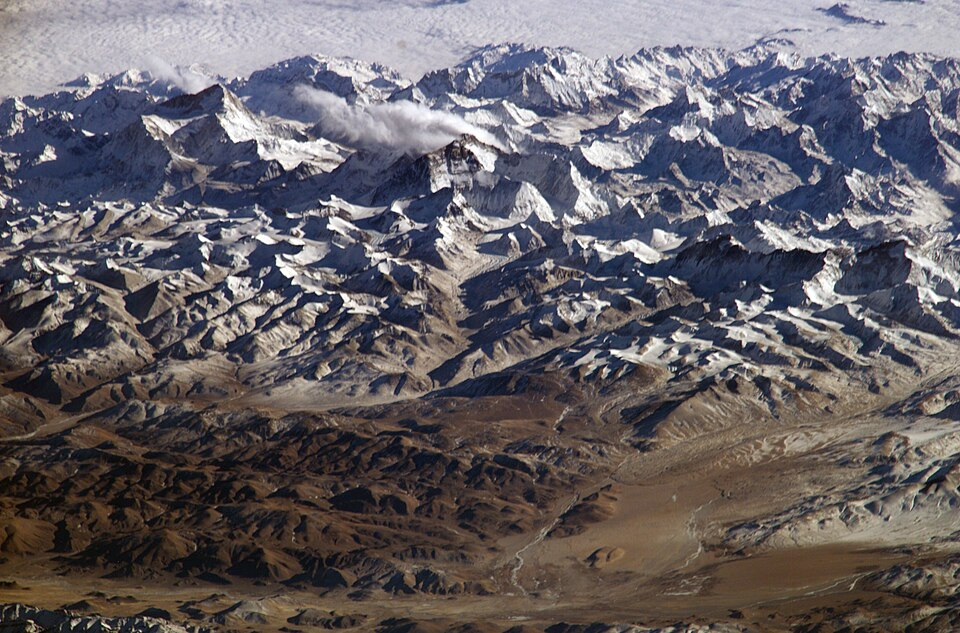
\includegraphics[width=0.75\linewidth]{images/book1/g4-himalaya-iss.jpg}

{\small O Himalaia visto da Estação Espacial Internacional, olhando para o
sul a partir do alto planalto do Tibete: um \omterm{def:g2:water-on-earth:ocean}{mar} de picos cobertos de \omterm{def:g4:clouds-rain-snow:precipitation}{neve}.
Foto: NASA (domínio público).}
% ledger: nasa:himalaya-iss
\end{omfigure}

\section{Os grandes rios e lagos}

A \omterm{def:g4:clouds-rain-snow:precipitation}{chuva} e a \omterm{def:g4:clouds-rain-snow:precipitation}{neve} derretida escorrem pela terra, juntam-se em riachos e
depois em \omterm{def:g1:landscapes-around-us:water}{rios}, e os \omterm{def:g1:landscapes-around-us:water}{rios} levam a água até o \omterm{def:g2:water-on-earth:ocean}{mar}. Os maiores \omterm{def:g1:landscapes-around-us:water}{rios} drenam
regiões inteiras de um \omterm{def:g3:continents-and-oceans:continent}{continente}.

Os dois \omterm{def:g1:landscapes-around-us:water}{rios} mais compridos da Terra são o Nilo, na África, e o Amazonas,
na América do Sul. Cada um tem perto de 7\,000 quilômetros. Qual é o mais
comprido? Ninguém concorda com certeza, porque isso depende de onde se
decide que um \omterm{def:g1:landscapes-around-us:water}{rio} começa: entre todos os riachos que se juntam para
formá-lo, qual conta como o seu verdadeiro começo? Em 2007, uma equipe que
seguiu o Amazonas até uma nascente mais distante disse que ele tinha cerca
de 6\,800 quilômetros, um pouco mais que o Nilo; muitas obras de
referência ainda dizem que o Nilo é o mais comprido.
% ledger: natgeo:nile, natgeo:amazon-nile-2007

O Amazonas é, sem nenhuma dúvida, o maior \omterm{def:g1:landscapes-around-us:water}{rio}: ele leva mais água que
qualquer outro.
% ledger: natgeo:amazon-nile-2007

\begin{omfigure}
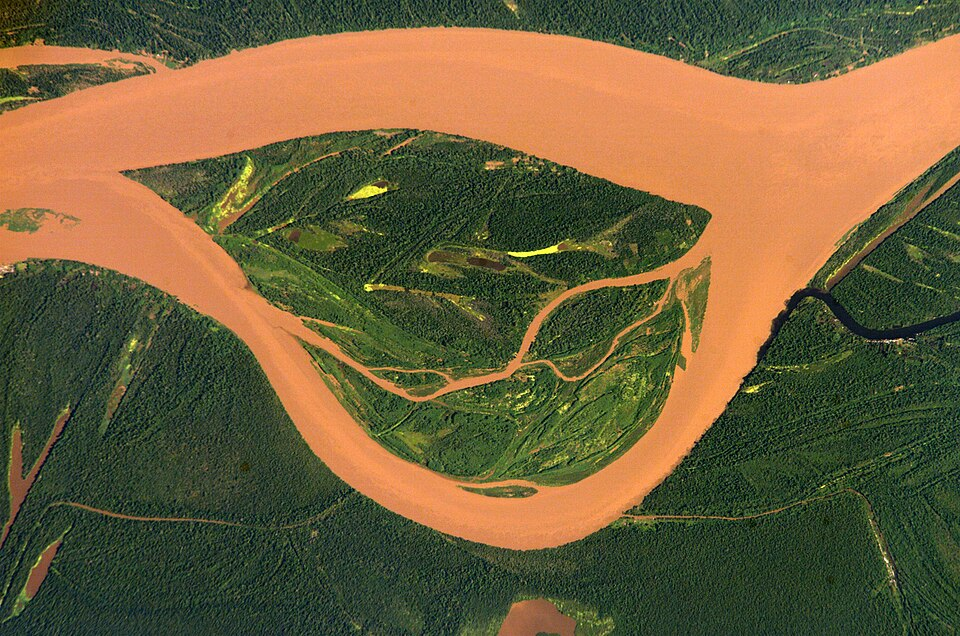
\includegraphics[width=0.6\linewidth]{images/book1/g4-amazon-iss.jpg}

{\small O Amazonas, marrom de \omterm{def:g3:stones-pebbles-sand:sand}{lama}, serpenteando pela floresta tropical,
visto da Estação Espacial Internacional. Foto: NASA (domínio público).}
% ledger: nasa:amazon-iss
\end{omfigure}

Os \omterm{def:g1:landscapes-around-us:water}{lagos} também batem recordes. O maior \omterm{def:g1:landscapes-around-us:water}{lago} da Terra é o \omterm{def:g2:water-on-earth:ocean}{mar} Cáspio,
entre a Europa e a Ásia: ele é tão grande que é chamado de \omterm{def:g2:water-on-earth:ocean}{mar}, mas está
fechado por terra de todos os lados. Ele cobre mais de 370\,000
quilômetros quadrados. O \omterm{def:g1:landscapes-around-us:water}{lago} mais profundo é o \omterm{def:g1:landscapes-around-us:water}{lago} Baikal, na Rússia:
em alguns lugares, o seu fundo fica a quase 2 quilômetros abaixo da superfície.
% ledger: natgeo:caspian-baikal

\section{Os desertos e os grandes gelos}

Dois tipos de lugar se destacam no \omterm{def:g4:world-physical-map:physical-map}{mapa físico} porque quase nada cresce
neles: os grandes desertos, onde quase nunca chove, e os grandes gelos.

O Saara, no norte da África, é o maior deserto quente da Terra. Ele cobre
cerca de oito milhões e meio de quilômetros quadrados. A África inteira
cobre cerca de 30 milhões de quilômetros quadrados; então o Saara é um
pouco mais que um quarto do \omterm{def:g3:continents-and-oceans:continent}{continente}: mais que $\frac{1}{4}$, mas menos
que $\frac{1}{3}$.
% ledger: natgeo:sahara, data:etopo1

Os grandes gelos cobrem a Antártida, em volta do \omterm{def:g3:continents-and-oceans:poles}{Polo Sul}, e a maior parte
da Groenlândia, no extremo norte do Atlântico. Ali, a \omterm{def:g4:clouds-rain-snow:precipitation}{neve} de milhares de
anos se acumulou e virou uma camada grossa de gelo. No \omterm{def:g4:world-physical-map:physical-map}{mapa físico}, as
cores dessas regiões são as das terras altas, porque o topo do gelo fica
bem acima do \omterm{def:g4:world-physical-map:altitude}{nível do mar}.

\section{O mais alto e o mais profundo}

O \omterm{def:g4:world-physical-map:physical-map}{mapa físico} mostra a forma da superfície da Terra, mas é tão pequeno que
esconde os extremos. Vamos colocá-los lado a lado, em escala.

\begin{omfigure}
\begin{tikzpicture}[x=1cm, y=0.32cm, font=\small]
  % sea level
  \fill[omHypsSeaA] (0,0) rectangle (9,-11.5);
  \fill[omHypsSeaD!80] (4.6,-11.5) -- (4.6,-11.0) -- (5.0,-10.98) -- (5.4,-11.0) -- (5.4,-11.5) -- cycle;
  \draw[black!60] (-0.2,0) -- (9.2,0);
  \node[anchor=west, font=\scriptsize] at (9.25,0) {nível do mar, 0\,m};
  % height scale
  \draw[black!60] (0,-11.5) -- (0,10);
  \foreach \h in {-10,-8,...,8} {
    \draw[black!60] (-0.1,\h) -- (0,\h);
    \node[anchor=east, font=\scriptsize] at (-0.12,\h) {\h\,km};
  }
  % ocean floor and trench
  \fill[brown!45] (0.05,-11.5) -- (0.05,-3.7) -- (3.2,-3.7) -- (4.4,-6) -- (4.9,-10.98) -- (5.1,-10.98)
    -- (5.6,-6) -- (6.4,-3.7) -- (9,-3.7) -- (9,-11.5) -- cycle;
  \node[font=\scriptsize, align=center] at (2.0,-5.3) {fundo do oceano,\\cerca de 3\,700\,m de profundidade};
  \node[font=\scriptsize, anchor=west, align=left] at (5.6,-9.4) {o ponto mais profundo:\\Depressão Challenger,\\quase 11\,000\,m};
  % Everest
  \fill[black!35] (6.6,0) -- (7.6,8.85) -- (8.6,0) -- cycle;
  \fill[white, draw=black!45, line width=0.3pt] (7.35,6.6) -- (7.6,8.85) -- (7.85,6.6) -- (7.6,7.1) -- cycle;
  \node[font=\scriptsize, align=center, anchor=south] at (7.6,8.95) {monte Everest, 8\,849\,m};
  % cirrus clouds band
  \draw[black!45, line width=0.6pt] (1.0,9.0) .. controls (1.6,9.5) and (2.2,9.1) .. (2.8,9.6);
  \draw[black!45, line width=0.6pt] (1.2,8.3) .. controls (1.8,8.8) and (2.4,8.4) .. (3.0,8.9);
  \node[font=\scriptsize, align=center] at (2.0,7.2) {nuvens altas\\(cirros)};
  % a village
  \fill[black!60] (2.2,1.5) rectangle (2.45,1.75);
  \node[font=\scriptsize, anchor=west] at (2.5,1.6) {uma vila na montanha, 1\,500\,m};
\end{tikzpicture}

{\small Do ponto mais profundo do \omterm{def:g2:water-on-earth:ocean}{oceano} até o pico mais alto, em escala. A
Depressão Challenger, no \omterm{def:g2:water-on-earth:ocean}{oceano} Pacífico, fica mais funda abaixo do \omterm{def:g2:water-on-earth:ocean}{mar} do
que o monte Everest se eleva acima dele. Valores: Everest 8\,849\,m;
Depressão Challenger quase 11\,000\,m; fundo médio do \omterm{def:g2:water-on-earth:ocean}{oceano} cerca de
3\,700\,m.}
\label{fig:g4:world-physical-map:extremes}
% ledger: tht:everest, usgs:trench-depth, nos:ocean-depth, wmo:cloud-levels
\end{omfigure}

\begin{example}[O Everest no fundo do mar]\label{ex:g4:world-physical-map:everest-in-deep}
Se pudéssemos levantar o monte Everest e colocá-lo no fundo da Depressão
Challenger, o seu pico ainda ficaria embaixo da água: cerca de 11\,000
metros de fossa, contra 8\,849 metros de \omterm{def:g1:landscapes-around-us:landform}{montanha}. Mais de 2 quilômetros
de \omterm{def:g2:water-on-earth:ocean}{mar} ainda o cobririam.
% ledger: tht:everest, usgs:trench-depth
\end{example}

\section{Exercícios}

\begin{exercise}[$\star$]\label{exo:g4:world-physical-map:1}
O que é a \omterm{def:g4:world-physical-map:altitude}{altitude} de um lugar? A partir de que nível ela é medida?
\end{exercise}

\begin{exercise}[$\star$]\label{exo:g4:world-physical-map:2}
Usando a \omterm{def:g2:drawing-to-map:legend}{legenda} do \omterm{def:g4:world-physical-map:physical-map}{mapa físico}, dê a \omterm{def:g4:world-physical-map:altitude}{altitude} de um lugar pintado de:
(a) verde-escuro; (b) amarelo-claro; (c) quase branco.
\end{exercise}

\begin{exercise}[$\star$]\label{exo:g4:world-physical-map:3}
Em que \omterm{def:g3:continents-and-oceans:continent}{continente} ficam: (a) os Andes; (b) o Himalaia; (c) o Saara;
(d) as \omterm{def:g1:landscapes-around-us:landform}{Montanhas} Rochosas?
\end{exercise}

\begin{exercise}[$\star$]\label{exo:g4:world-physical-map:4}
Diga o nome da \omterm{def:g1:landscapes-around-us:landform}{montanha} mais alta da Terra, do maior \omterm{def:g1:landscapes-around-us:water}{lago} e do \omterm{def:g1:landscapes-around-us:water}{lago} mais profundo.
\end{exercise}

\begin{exercise}[$\star$]\label{exo:g4:world-physical-map:5}
No \omterm{def:g4:world-physical-map:physical-map}{mapa físico}, o \omterm{def:g2:water-on-earth:ocean}{mar} perto das costas é azul-claro, e o meio dos \omterm{def:g2:water-on-earth:ocean}{oceanos} é
azul-escuro. O que isso diz sobre a profundidade do \omterm{def:g2:water-on-earth:ocean}{mar}?
\end{exercise}

\begin{exercise}[$\star$]\label{exo:g4:world-physical-map:6}
Por que a Antártida e a Groenlândia estão pintadas como terras altas no
\omterm{def:g4:world-physical-map:physical-map}{mapa físico}?
\end{exercise}

\begin{exercise}[$\star\star$]\label{exo:g4:world-physical-map:7}
Coloque em ordem, do mais baixo para o mais alto: uma praia; uma vila a
1\,500 metros; o topo do monte Everest; o fundo da Depressão Challenger;
o fundo médio do \omterm{def:g2:water-on-earth:ocean}{oceano}.
\end{exercise}

\begin{exercise}[$\star\star$]\label{exo:g4:world-physical-map:8}
Por que não podemos dizer com certeza se o Nilo ou o Amazonas é o \omterm{def:g1:landscapes-around-us:water}{rio} mais
comprido?
\end{exercise}

\begin{exercise}[$\star\star$]\label{exo:g4:world-physical-map:9}
A África cobre cerca de 30 milhões de quilômetros quadrados. Quanto é um
quarto disso? E um terço? O Saara cobre cerca de oito milhões e meio de
quilômetros quadrados: isso é mais ou menos que um quarto da África? Mais
ou menos que um terço?
\end{exercise}

\begin{exercise}[$\star\star$]\label{exo:g4:world-physical-map:10}
Um abrigo de \omterm{def:g1:landscapes-around-us:landform}{montanha} fica a 2\,500 metros, e um \omterm{def:g1:landscapes-around-us:water}{lago} abaixo dele a 1\,000
metros. Quantos metros mais alto fica o abrigo? Que cores eles têm no \omterm{def:g4:world-physical-map:physical-map}{mapa
físico}?
\end{exercise}

\begin{exercise}[$\star\star\star$]\label{exo:g4:world-physical-map:11}
Um avião voa a 10 quilômetros acima do \omterm{def:g4:world-physical-map:altitude}{nível do mar}. Ele está mais alto
que o monte Everest? Quantos metros mais alto? Se ele voasse sobre a
Depressão Challenger, a que distância do fundo da fossa ele estaria (use
11\,000 metros para a fossa)?
\end{exercise}
